% -*- latex -*-
%%%%%%%%%%%%%%%%%%%%%%%%%%%%%%%%%%%%%%%%%%%%%%%%%%%%%%%%%%%%%%%%
%%%%
%%%% This TeX file is part of the course
%%%% Introduction to Scientific Programming in C++/Fortran2003
%%%% copyright 2017/8 Victor Eijkhout eijkhout@tacc.utexas.edu
%%%%
%%%% algodata.tex : introductin to algorithms and data structures
%%%%
%%%%%%%%%%%%%%%%%%%%%%%%%%%%%%%%%%%%%%%%%%%%%%%%%%%%%%%%%%%%%%%%

\Level 0 {Data structures}

The main data structure you have seen so far is the array. In this
section we briefly sketch some more complicated data structures.

\Level 1 {Stack}
\index{stack|(textbf}

A \emph{stack} is a data structure that is a bit like an
array, except that you can only see the last element:
\begin{itemize}
\item You can inspect the last element;
\item You can remove the last element; and
\item You can add a new element that then becomes the last element;
  the previous last element becomes invisible: it becomes visible
  again as the last elememt if the new last element is removed.
\end{itemize}
The actions of adding and removing the last element are known as
\indexterm{push} and \indexterm{pop} respectively.

\begin{exercise}
  Write a class that implements a stack of integers. It should have
  methods
\begin{verbatim}
void push(int value);
int pop();
\end{verbatim}
\end{exercise}

\index{stack|)}

\Level 1 {Linked lists}
\index{list!linked|(textbf}
\label{sec:linklist}

\prerequisite{\ref{ch:pointer}}

Arrays are not flexible: you can not insert an element in the
middle. Instead:
\begin{itemize}
\item Allocate a larger array,
\item copy data over (with insertion),
\item delete old array storage
\end{itemize}
This is expensive. (It's what happens in a
C++~\indextermtt{vector}; section~\ref{sec:stdvector-dynamic}.)

\begin{figure}[ht]
\hbox{%
  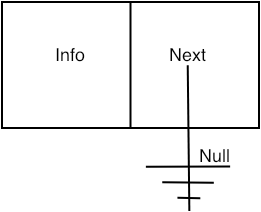
\includegraphics[scale=.3]{linkednode}
  \
  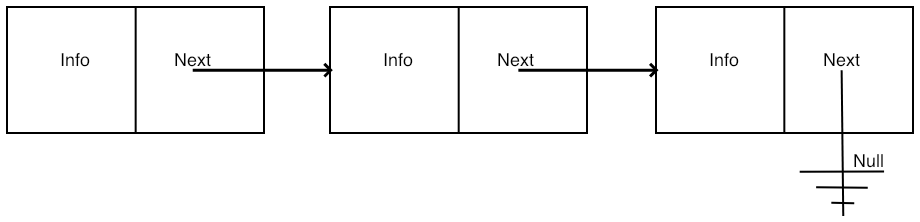
\includegraphics[scale=.3]{linkedlist}
  }
  \caption{Node data structure and linked list of nodes}
  \label{fig:linked-node-list}
\end{figure}

If you need to do lots of insertions, make a
\emph{linked list}. The basic data structure is a \n{Node},
which contains 
\begin{enumerate}
\item
  Information, which can be anything; and
\item A pointer (sometimes called `link') to the next node. If there
  is no next node, the pointer will be \n{NULL}. Every language has
  its own way of denoting a \indextermsub{null}{pointer}.
\end{enumerate}
\verbatimsnippet{linklist}

We illustrate this in figure~\ref{fig:linked-node-list}.

\begin{figure}[ht]
  \hbox{
  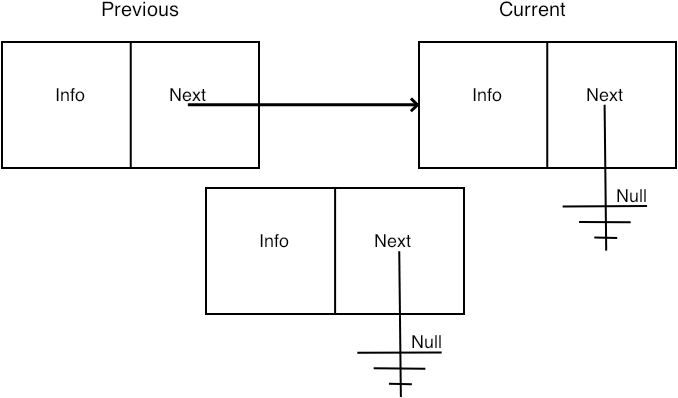
\includegraphics[scale=.3]{linkedinsert1}
  \
  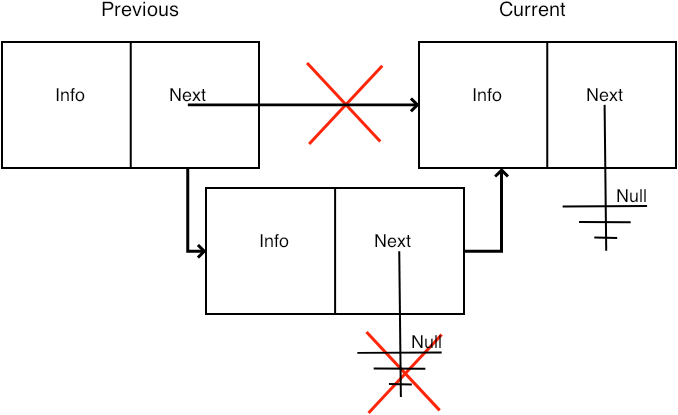
\includegraphics[scale=.3]{linkedinsert2}
  }
  \caption{Insertion in a linked list}
  \label{fig:linked-list-insert}
\end{figure}

The obvious operations on a linked list are searching for an element,
and inserting a new element. See figure~\ref{fig:linked-list-insert}.

%\verbatimsnippet{linkinsert}

We declare the basic classes. A~node has information fields, and a
link to another node:
%
\verbatimsnippet{linknode}

A linked list has as its only member a pointer to a node:
%
\verbatimsnippet{linklist}

Many list algorithms consist of going down the links:
%
\verbatimsnippet{listcontains}

The interesting methods are of course those that alter the
list. Inserting a new value in the list has basically two cases:
\begin{enumerate}
\item If the list is empty, create a new node, and set the head of the
  list to that node.
\item If the list is not empty, we have several more cases, depending
  on whether the value goes at the head of the list, the tail,
  somewhere in the middle. And we need to check whether the value is
  already in the list.
\end{enumerate}
The second case is tricky. We make the following design: there is a
routine that takes a node, possibly with other nodes tailing, and it
gives back the same node or another node, so that the new node plus
its tail have all the previous information plus the new one.
\begin{verbatim}
shared_ptr<Node> Node::insert(int value);
\end{verbatim}

There are a lot of cases here. You can try this by an approach called
\acf{TDD}: first you decide on a test, then you write the code that
covers that case.

\begin{exercise}
  Write a \n{List::length} method, so that this code gives the right
  output:
  %
  \verbatimsnippet{liststep1}
\end{exercise}

\begin{exercise}
  Next write the case of \n{Node::insert} that handles the empty
  list. You also need a method \n{List::contains} that tests if an
  item if in the list.
  %
  \verbatimsnippet{liststep2}
\end{exercise}

\begin{exercise}
  Inserting a value that is already in the list means that the
  \n{count} value of a node needs to be increased. Update your
  \n{insert} method to make this code work:
  %
  \verbatimsnippet{liststep3}
\end{exercise}

\begin{exercise}
  One of the remaining cases is inserting an element that goes at the
  head. Update your \n{insert} method to get this to work:
  %
  \verbatimsnippet{liststep4}
\end{exercise}

\begin{exercise}
  Finally, if an item goes at the end of the list:
  %
  \verbatimsnippet{liststep5}
\end{exercise}

\index{list!linked|)}

\Level 1 {Trees}

\prerequisite{\ref{ch:pointer}}

A tree can be defined recursively:
\begin{itemize}
\item A tree is empty, or
\item a tree is a node with some number of children trees.
\end{itemize}
Let's design a tree that stores and counts integers: each node has a
label, namely an integer, and a count value that records how often we
have seen that integer.

Our basic data structure is the node, and we define it recursively to
have up to two children. This is a problem: you can not write
\begin{verbatim}
class Node {
private:
  Node left,right;
}
\end{verbatim}
because that would recursively need infinite memory. So instead we use pointers.
%
\verbatimsnippet{treenode}
%
and we record that we have seen the integer zero zero times.

Algorithms on a tree are typically recursive. For instance, the total
number of nodes is computed from the root. At any given node, the
number of nodes of that attached subtree is one plus the number of
nodes of the left and right subtrees.
%
\verbatimsnippet{treecount}

Likewise, the depth of a tree is computed as a recursive max over the
left and right subtrees:
%
\verbatimsnippet{treedepth}

Now we need to consider how actually to insert nodes. We write a
function that inserts an item at a node. If the key of that node is
the item, we increase the value of the counter. Otherwise we determine
whether to add the item in the left or right subtree. If no such
subtree exists, we create it; otherwise we descend in the appropriate
subtree, and do a recursive insert call.
%
\verbatimsnippet{treeinsert}

\Level 0 {Algorithms}

This \emph{really} \textbf{really} goes beyond this book.

\begin{itemize}
\item Simple ones: numerical
\item Connected to a data structure: search
\end{itemize}

\Level 1 {Sorting}

Unlike the tree algorithms above, which used a non-obvious data
structure,
sorting algorithms are a good example of the combination of very
simple data structures (mostly just an array), and sophisticated
analysis of the algorithm behaviour. We very briefly discuss two
algorithms.

\Level 2 {Bubble sort}

An array $a$ of length~$n$ is sorted if
\[ \forall_{i<n-1}\colon a_i\leq a_{i+1}. \]
A simple sorting algorithm suggests itself immediately: if $i$ is such
that $a_i>a_{i+1}$, then reverse the $i$ and $i+1$ locations in the
array.

\verbatimsnippet{swaplocs}

(Why is the array argument passed by reference?)

If you go through the array once, swapping elements, the result is not
sorted, but at least the largest element is at the end. You can now do
another pass, putting the next-largest element in place, and so on.

This algorithm is known as \indexterm{bubble sort}. It is generally
not considered a good algorithm, because it has a time complexity
(section~\ref{sec:time_complex}) of $n^2/2$ swap operations. Sorting
can be shown to need $O(n\log n)$ operations, and bubble sort is far
above this limit.

\Level 2 {Quicksort}

A popular algorithm that can attain the optimal complexity (but need
not; see below) is \indexterm{quicksort}:
\begin{itemize}
\item Find an element, called the pivot, that is approximately equal
  to the median value.
\item Rearrange the array elements to give three sets, consecutively
  stored: all elements less than, equal, and greater than the pivot
  respectively.
\item Apply the quicksort algorithm to the first and third subarrays.
\end{itemize}

This algorithm is best programmed recursively, and you can even make a
case for its parallel execution: every time you find a pivot you can
double the number of active processors.

\begin{exercise}
  Suppose that, by bad luck, your pivot turns out to be the smallest
  array element every time. What is the time complexity of the
  resulting algorithm?
\end{exercise}

\Level 0 {Programming techniques}

\Level 1 {Memoization}
\label{sec:memo}

In section~\ref{sec:recursion} you saw some examples of recursion. The
factorial example could be written in a loop, and there are both arguments
for and against doing so. 

The Fibonacci example is more subtle: it can not immediately be
converted to an iterative formulation, but there is a clear need for
eliminating some waste that comes with the simple recursive
formulation. The technique we can use for this is known as
\indextermdef{memoization}: store intermediate results to prevent them
from being recomputed.

Here is an outline.
\verbatimsnippet{fibomemo}
